%
%===============>>  ГРУППА 11-5 МОДУЛЬ 4  <<=============
%
\setmodule{4}
%
%===============>>  Занятие 1  <<===============
%
\begin{class}[number=1]
	\begin{listofex}
		\item Упростить:
		\begin{enumcols}[itemcolumns=4]
			\item \( \sin(90\degree-x) \)
			\item \( \cos(360\degree + x) \)
			\item \( \tg(180\degree+x) \)
			\item \( \cos(810\degree-x) \)
		\end{enumcols}
		\item Вычислить:
		\begin{enumcols}[itemcolumns=2]
			\item \( \dfrac{\sqrt{3}}{\sin60\degree}+\dfrac{3}{\sin30\degree} \)
			\item \( \dfrac{17\sin155\degree}{\sin25\degree} \)
			\item \( \dfrac{-2\sin105\degree}{\cos15\degree} \)
			\item \( \sin^215\degree-1+\cos^215 \)
			\item \( -\sqrt{27}\cos30\degree-\sqrt{2}\sin45\degree\ctg60\degree\tg60\degree\)
			\item \( \dfrac{9\sin45\degree\cos45\degree}{\cos^245\degree-\sin^245\degree} \)
		\end{enumcols}
		\item Вычислить:
		\begin{enumcols}[itemcolumns=2]
			\item \( \sin240\degree\sin150\degree\sin(-90)\degree\tg30\degree \)
			\item \( \cos(-300\degree)\sin(-120\degree)\tg(-150\degree) \)
		\end{enumcols}
		\item Упростить:
		\begin{enumcols}[itemcolumns=4]
			\item \( \sin\left( \dfrac{\pi}{2}+x \right) \)
			\item \( \cos(\pi+x) \)
			\item \( \tg\left( \dfrac{3\pi}{2}-x \right) \)
			\item \( \sin(-3,5\pi-x) \)
		\end{enumcols}
		\item Вычислить:
		\begin{enumcols}[itemcolumns=2]
			\item \( \sin\dfrac{5\pi}{4}\cos\dfrac{4\pi}{3}\tg\dfrac{2\pi}{3}\ctg\dfrac{3\pi}{4} \)
			\item \( \cos\left( -\dfrac{5\pi}{3} \right)\sin\left( -\dfrac{5\pi}{2} \right)\sin\dfrac{3\pi}{2} \)
		\end{enumcols}
		\item Вычислить:
		\begin{enumcols}[itemcolumns=2]
			\item \( \sin\dfrac{\pi}{4}\cos\dfrac{\pi}{6}\tg\dfrac{\pi}{3} \)
			\item \( \cos\left( -\dfrac{\pi}{2} \right)+\sqrt{3}\sin\left( -\dfrac{\pi}{3} \right) \)
			\item \( \sin(-2\pi)+0,23\cos\left( \dfrac{3\pi}{2} \right) \)
			\item \( \sin\left( \dfrac{3\pi}{4} \right)+\cos\left( -\dfrac{5\pi}{6} \right) \)
			\item \( \ctg\left( \dfrac{3\pi}{2} \right)+\dfrac{1}{\sqrt{2}}\sin\left( \dfrac{5\pi}{4} \right) \)
			\item \( \sin(-2,5\pi)-(3\cos(-\pi))^2 \)
		\end{enumcols}
		\item Упростить выражение:
		\begin{enumcols}[itemcolumns=1]
			\item \( \ctg\left( \dfrac{3\pi}{2}+x \right)\ctg(\pi-x)-\ctg\left( \dfrac{\pi}{2}+x \right)\tg(2\pi+x) \)
			\item \( \cos\left( \dfrac{3\pi}{2}+x \right)\sin x + \sin^2(3\pi+x)+\tg(5\pi+x)\ctg x \)
			\item \( \dfrac{\sin x}{1+\cos x}+\ctg x \)
		\end{enumcols}
	\end{listofex}
\end{class}
%
%===============>>  Занятие 2  <<===============
%
%\begin{class}[number=2]
%	\begin{listofex}
%		\item Пусто
%	\end{listofex}
%\end{class}
%
%===============>>  Домашняя работа 1  <<===============
%
\begin{homework}[number=1]
	\begin{listofex}
		\item Вычислить:
		\begin{enumcols}[itemcolumns=2]
			\item \( \dfrac{\sqrt{3}}{\tg60\degree}+\dfrac{9}{\sin30\degree} \)
			\item \( \dfrac{19\sin214\degree}{\sin34\degree} \)
			\item \( \dfrac{-10\sin115\degree}{\cos25\degree} \)
			\item \( \sin^2126\degree-2+\cos^2126\degree \)
		\end{enumcols}
		\item Вычислить с помощью формул синуса/косинуса двойного угла:
		\begin{enumcols}[itemcolumns=2]
			\item \( 2\sin\dfrac{\pi}{8}\cos\dfrac{\pi}{8} \)
			\item \( \cos^215\degree-\sin^215\degree \)
			\item \( 10\sin75\degree\cos75\degree \)
			\item \( \sqrt{27}\cos^2\dfrac{13\pi}{2}-\sqrt{27}\sin^2\dfrac{13\pi}{12} \)
		\end{enumcols}
		\item Вычислите с помощью метода приведения:
		\begin{enumcols}[itemcolumns=6]
			\item \( \sin600\degree \)
			\item \( \tg480\degree \)
			\item \( \cos330\degree \)
			\item \( \sin240\degree \)
			\item \( \cos\dfrac{9\pi}{4} \)
			\item \( \sin\dfrac{7\pi}{4} \)
			\item \( \cos\dfrac{3\pi}{2} \)
			\item \( \tg\dfrac{7\pi}{6} \)
		\end{enumcols}
	\item Одного рулона обоев хватает для оклейки полосы от пола до потолка шириной \( 1,3 \) м. Сколько рулонов обоев нужно купить для оклейки прямоугольной комнаты размерами \(  2,1 \) м на \( 5,9 \) м?
	\item Найдите значение выражения: \( \left( -\mfrac{2}{3}{4}-\dfrac{3}{8} \right)\cdot160 \)
	\end{listofex}
\end{homework}
%
%===============>>  Занятие 3  <<===============
%
\begin{class}[number=3]
	\begin{listofex}
		\item 	
		\begin{enumcols}[itemcolumns=1]
			\item \exercise{1117}
			\item \exercise{1118}
			\item \exercise{1119}
			\item \exercise{2965}
			\item \exercise{2874}
			\item \exercise{2865}
			\item \exercise{2934}
			\item \exercise{1808}
			\item \exercise{1809}
		\end{enumcols}
		\item В летнем лагере на каждого участника полагается \( 30 \) г сахара в день. В лагере \( 103 \) человека. Сколько килограммовых упаковок сахара понадобится на весь лагерь на \( 6 \) дней?
		\item В доме, в котором живёт Женя, один подъезд. На каждом этаже по восемь квартир. Женя живёт в квартире \( 87 \). На каком этаже живёт Женя?
		\item Длину окружности \( l \) можно вычислить по формуле \( l=2\pi R \), где \( R \) -- радиус окружности (в метрах). Пользуясь этой формулой, найдите радиус окружности, если её длина равна \( 78 \) м. (Считать \( \pi=3 \)).
		\item Площадь трапеции \( S \) (в м\( ^2 \)) можно вычислить по формуле \( S=\dfrac{a+b}{2}\cdot h \),  где \( a\), \( b   \) -- основания трапеции, \( h \) -- высота (в метрах). Пользуясь этой формулой, найдите высоту \( h \), если основания трапеции равны \( 5 \) м   и \( 7 \) м, а её площадь \( 24 \) м\( ^2 \).
	\end{listofex}
\end{class}
%
%===============>>  Занятие 4  <<===============
% смещение на одно занятие с прошлого месяца
\begin{exam}
	\begin{listofex}
		\item Напишите основное тригонометрическое тождество
		\item Что такое тангенс в прямоугольном треугольнике? (отношение...)
		\item Что такое косинус в прямоугольном треугольнике? (отношение...)
		\item Вычислить:
			\begin{tasks}(2)
				\task \( 37\cos450\degree \)
				\task \( 20\sin120\degree\cos150\degree \)
				\task \( 20\sqrt{30\tg390\degree} \)
				\task \( \dfrac{12\sin11\degree\cdot\cos11\degree}{\sin22\degree} \)
				\task \( \dfrac{8}{\sin\left( -\dfrac{27\pi}{4} \right)\cos\left( \dfrac{31\pi}{4} \right)} \)
				\task \( \dfrac{12}{\sin^227\degree+\cos^2207\degree} \)
				\task \( \dfrac{5\sin74\degree}{\cos37\degree\cdot\cos53\degree} \)
			\end{tasks}
		\item Найдите \(\cos\alpha\),\quad если \( \sin \alpha = -0,6 \) и \( 180\degree<\alpha<270\degree \)
		\item Найдите \( \tg\alpha \), \quad если \( \cos\alpha=\dfrac{2}{\sqrt{5}} \) и \( \alpha\in\left( \dfrac{3\pi}{2};2\pi \right) \)
		\item Теплоход рассчитан на \( 700  \) пассажиров и \( 20 \) членов команды. Каждая спасательная шлюпка может вместить \( 70 \) человек. Какое наименьшее число шлюпок должно быть на теплоходе, чтобы в случае необходимости в них можно было разместить всех пассажиров и всех членов команды?
		\item В треугольнике \( ABC \) \( AC = BC = 25 \), \( AB = 40 \). Найдите  \( \sin A \).
		\item
		\begin{minipage}[t]{0.57\textwidth}
			 В треугольнике \( ABC \) стороны \( AC  \) и \( BC  \) равны. Внешний угол при вершине \( B \) равен \( 125\degree\). Найдите угол \( C \). Ответ дайте в градусах.
		\end{minipage}
		\begin{minipage}[c]{0.3\textwidth}
			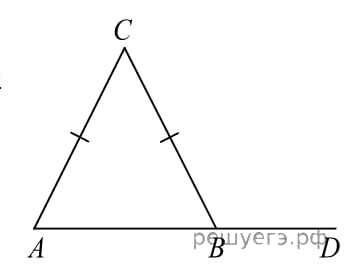
\includegraphics[align=t, width=\textwidth]{pics/G115M4L4-1}
		\end{minipage}
	\end{listofex}
\end{exam}
%
%===============>>  Домашняя работа 2  <<===============
%
\begin{homework}[number=2]
	\begin{listofex}
		\item По тарифному плану «Просто как день» компания сотовой связи каждый вечер снимает со счёта абонента \( 18 \) руб. Если на счету осталось меньше \( 18 \) руб., то на следующее утро номер блокируют до пополнения счёта. Сегодня утром у Лизы на счету было \( 800 \) руб. Сколько дней (включая сегодняшний) она сможет пользоваться телефоном, не пополняя счёт?
		\item Баночка йогурта стоит \( 14 \) рублей \( 60 \) копеек. Какое наибольшее количество баночек йогурта можно купить на \( 100 \) рублей?
		\item Стоимость проезда в маршрутном такси составляет \( 20 \) руб. Какое наибольшее число поездок можно будет совершить в этом маршрутном такси на \( 150 \) руб., если цена проезда снизится на \( 10\% \)?
		\item Найдите \( 3\sqrt{2}\sin x \), \quad если \( \cos x=\dfrac{1}{3} \) и \( x\in\left( 0;\dfrac{\pi}{2} \right) \)
		\item Вычислите:
		\begin{tasks}(3)
			\task \( (728^2-26^2):754\)
			\task \( \dfrac{2}{5}+\dfrac{1}{4}+3 \)
			\task \( 0,86:\dfrac{43}{20} \)
			\task \( \dfrac{4}{11}:\left( -\dfrac{16}{33} \right)+\mfrac{5}{3}{4} \)
			\task \( \dfrac{(2\sqrt{7})^2}{14} \)
			\task \( (\sqrt{13}-2\sqrt{3})(\sqrt{13}+2\sqrt{3}) \)
		\end{tasks}
		\item Площадь четырехугольника S (в м\( ^2 \)), можно вычислить по формуле \( S=\dfrac{1}{2}d_1d_2\sin\alpha \),  где \( d_1 \) и \( d_2 \) --- длины диагоналей четырехугольника, \( \alpha \) --- угол между диагоналями. Пользуясь этой формулой, найдите площадь \( S \), если \( d_1=4 \), \( d_2=3  \) и \( \sin\alpha=\dfrac{5}{6} \).
	\end{listofex}
\end{homework}
%
%===============>>  Занятие 5  <<===============
% смещение на одно занятие с прошлого месяца
%\begin{class}[number=5]
%	\begin{listofex}
%		\item Пусто
%	\end{listofex}
%\end{class}
%
%===============>>  Домашняя работа 3  <<===============
%
%\begin{homework}[number=2]
%	\begin{listofex}
%
%	\end{listofex}
%\end{homework}
%\newpage
%\title{Подготовка к проверочной работе}
%\begin{listofex}
%	
%\end{listofex}
%
%===============>>  Занятие 7  <<===============
%
%\begin{class}[number=7]
%	\begin{listofex}
%	
%	\end{listofex}
%\end{class}
%
%===============>>  Провечная работа  <<===============
%
%\begin{exam}
%	\begin{listofex}
%	
%	\end{listofex}
%\end{exam}